\documentclass[]{beamer}
\usefonttheme[onlymath]{serif}
\setbeamertemplate{navigation symbols}{}
\usetheme{Frankfurt}
%\usecolortheme{rose}
\usecolortheme{seahorse}
\usepackage{tikz}
\usepackage{lipsum}

\usepackage{verbatim}
\usepackage{epsfig}

\newcommand{\blue}{\color{blue}}
\newcommand{\red}{\color{red}}
\def\octave{\texttt{octave }}
\def\lapack{\texttt{lapack }}
\def\gnuplot{\texttt{gnuplot}}
\def\t#1{{\texttt{#1}}}
\def\vr{\vec{r}}

%\usepackage{beamerthemesplit}
%\usetheme{CambridgeUS}
\setbeamertemplate{navigation symbols}{}

\author{Yavar T Azar}
\institute{Nuclear Science and technology research institute (NSTRI)}

\date{04 May 2019}

\title{Introduction to Quantum-Espresso}


\titlegraphic{
\includegraphics[width=11cm]{logo}
}
\begin{document}
\begin{frame}
  \titlepage
\end{frame}

\begin{frame}
  \frametitle{Outline}
  \tableofcontents
\end{frame}

\section{Introduction}
\begin{frame}
\frametitle{Web-site introduction}
	\begin{figure}
	\centering
	
\includegraphics[width=0.5\linewidth]{QE_website}
	\label{fig:qewebsite}
\end{figure}
\begin{block}{}\small
Quantum ESPRESSO is an integrated suite of computer codes for
electronic-structure calculations and materials modeling at the
nanoscale. It is based on density-functional theory, plane waves, and
pseudopotentials (both norm-conserving and ultrasoft).
\end{block}
\begin{center}
\blue{Source : \texttt{http://www.quantum-espresso.org/}}
\end{center}
\begin{itemize}
\item {\blue{ESPRESSO}} = op{\blue{E}}n {\blue{S}}ource {\blue{P}}ackage
for {\blue{R}}esearch in {\blue{E}}lectronic {\blue{S}}tructure,
{\blue{S}}imulation, and {\blue{O}}ptimization
\item GNU General Public License
\end{itemize}
\end{frame}

\begin{frame}
\begin{itemize}
\item Codes under Quantum ESPRESSO
\begin{itemize}
\item PWSCF : Plane-wave self-consisten field
\item PP: Post-processing
\item CP : Car-Parrinello molecular dynamics
\item PHONON  : Phonon calculations
\item FPMD : Molecular Dynamics
\item Wannier
\end{itemize}
\item We'll mostly deal with PWSCF (pw.x). Other components have similar input
structure.
\end{itemize}
\end{frame}

\begin{frame}
\frametitle{Capabilities}
\begin{itemize}
\item Self-consistent, planewave, pseudopotential total energy calculation
\item Large xc library : LDA, GGA, BLYP, LDA+U
\item Pseudopotential-generation code and pseudopotential library
\begin{itemize}
\item Norm-conserving, ultrasoft
\item Scalar relativistic, fully relativistic
\end{itemize}
\end{itemize}
\end{frame}
]
\frame{text}
{ 

\textcolor{white}{...}
	\begin{itemize}
		\item Geometric optimization also with variable cells
		\item Phonon calculations, (harmonic/anharmonic/e-ph)
		\item Inclusion of electric field, macroscopic polarizability
		\item Noncollinear magnetism
		\item Infrared and Raman cross sections
		\item Dielectric tensors
		\item Metadynamics
		\item Ballistic conductance
		\item Maximally localized Wannier functions
		\item Nudged Elastic Bands (NEB)
		\end{itemize} 
\textcolor{white}{...}
}
\begin{frame}
\begin{itemize}
\item {\blue{Pros : }} 
\begin{itemize}
\item Free $\Rightarrow$ huge community  
\item Mature code, core is mostly well-tested 
\item MANY options, keywords 
\item Excellent mailing list, helpful developers
\end{itemize}
\item {\blue{Cons : }}
\begin{itemize}
\item 
\item Hard to read the code
\item Redundancies/obsolete keywords
\end{itemize}
\end{itemize}
\end{frame}


\section{The input}
\subsection{Namelists}
\begin{frame}
\frametitle{General structure}
\begin{itemize}
\item The input file is broken down into sections
\end{itemize}
\begin{block}{Namelists --- calculation specifications}
  \texttt{\&CONTROL}: general variables controlling the run\\
  \texttt{\&SYSTEM}: structural information on the system under investigation\\
  \texttt{\&ELECTRONS}: electronic variables\\
  \texttt{\&IONS} (optional): ionic variables\\
  \texttt{\&CELL} (optional): variable-cell dynamics\\
  \texttt{\&PHONON} (optional): information required to produce data for
  phonon calculations\\
\end{block}
\end{frame}

\begin{frame}
\frametitle{General structure}
\begin{block}{Nonoptional and optional cards}
  \texttt{ATOMIC SPECIES}\\
  \texttt{ATOMIC POSITIONS}\\
  \texttt{K\_POINTS}\\
  \texttt{CELL PARAMETERS}(optional)\\
  \texttt{OCCUPATIONS}(optional)\\
  \texttt{FIRST\_IMAGE}(optional)\\
  \texttt{LAST\_IMAGE}(optional)\\
  \texttt{CLIMBING IMAGES}(optional)\\
\end{block}
\end{frame}

\begin{frame}[fragile]
\begin{block}{Typical input file --- diamond GaAs}
\begin{tiny}
\begin{verbatim}
&CONTROL
calculation = 'scf' ,
outdir = './' ,
pseudo_dir = './' ,
prefix = 'GaAs1' ,
tprnfor = .true. ,
/
&SYSTEM
ibrav = 2,
celldm(1) = 10.866264585,
nat = 2, ntyp = 2,
ecutwfc = 30 , ecutrho = 240 ,
occupations = 'smearing' ,
/
&ELECTRONS
electron_maxstep = 200,
conv_thr = 1.0D-7 ,
mixing_mode = 'plain' , mixing_beta = 0.1D0 ,
mixing_ndim = 10,
diagonalization = 'david' ,
/
ATOMIC_SPECIES
Ga   69.72    ga_pbe_v1.4.uspp.F.UPF
As   74.92    as_pbe_v1.uspp.F.UPF

ATOMIC_POSITIONS crystal
Ga 0.00000 0.00000 0.00000
As 0.75000 0.75000 0.75000

K_POINTS automatics
3 3 3 0 0 0
\end{verbatim}
\end{tiny}
\end{block}
\begin{tikzpicture}[remember picture,overlay]
\node at (current page.center) {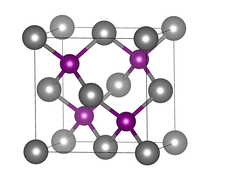
\includegraphics[width=4cm]{GaAs}};

\end{tikzpicture}

\end{frame}

\begin{frame}
\frametitle{The namelist \texttt{\&control} }
\begin{block}{General keywords}
\begin{itemize}
\item<1->\t{calculation} : 
\begin{itemize}
  \item[] \t{scf} : single point calculation without geometric optimization 
  \item[] \t{nscf} : non-self-consistent calculation (needs previous $V_{eff}(\vr)$)
  \item[] \t{relax} : geometric optimization
  \item[] \t{md} : molecular dynamics
  \item[] \t{vc-relax} : geometric optimization with variable unit cell
  coordinates
\end{itemize}
\item<2->\t{restart\_mode} :
\begin{itemize} 
\item[] \t{from\_scratch} : Start from an initial guess for the $\{\psi_i(\vr)\}$
\item[] \t{restart} : Start from earlier data \\
{\blue{Note 1}} : PWSCF writes to disk $n(\vr)$, $V_{eff}(\vr)$ and $\{\psi_i(\vr)\}$\\
{\blue{Note 2}} : Must interrupt properly to resume calculation.\\
\end{itemize}
\item<3-> \t{outdir} : Directory where intermediates are dumped.
\item<4-> \t{pseudo\_dir} : Directory where the pseudopotentials live.
\end{itemize}
\end{block}
\end{frame}

\begin{frame}
  \frametitle{The namelist \t{\&system}}
  \begin{block}{General keywords}
    \begin{itemize}
      \item<1-> \t{nat} : number of atoms
      \item<1-> \t{ntyp} : number of types of atoms
      \item<2-> \t{nbnd} : number of states to be calculated (unoccupied states
      as well)
      \item<3-> \t{ecutwfc} : kinetic energy cutoff (for planewaves)
      \item<3-> \t{ecutrho} : density cutoff (for the augmentation charge in
      USPP $\approx$ 10$\times$ \t{ecutwfc})
    \end{itemize}
  \end{block}
\end{frame}


\begin{frame}
  \frametitle{The namelist \t{\&system}}
  \begin{block}{Lattice structure}
    \begin{itemize}
    \item<1-> \t{ibrav} : Bravais lattice index --- easy way to set up a crystal
    \item<2-> \t{celldm(1)-celldm(6)} : Various cell dimensions in B --- not all six are
    used for most \t{ibrav} \\
    \begin{center}
      \begin{tabular} { l | l }
        0 : user-specified   &   \t{celldm(1)} = given length\\
        1 : simple cubic     &   \t{celldm(1)} = a \\
        2 : face-centered cubic & \t{celldm(1)} = a \\
        3 : body-centered cubic & \t{celldm(1)} = a \\
        4 : hexagonal & \t{celldm(1)} = a \\
        & \t{celldm(3)}=c/a\\
        $\quad$$\quad$$\quad$\vdots & $\quad$$\quad$$\quad$\vdots \\
        Up to fourteen & Some celldm(i) length, some angle \\
      \end{tabular}
    \end{center}
    \end{itemize}
  \end{block}
\end{frame}

\begin{frame}
  \frametitle{The namelist \t{\&system}}
  \begin{block}{Occupations}
    \begin{itemize}
    \item<1-> \t{occupations} : Occupation of Kohn-Sham states -- important
    for metals
      \begin{itemize}
        \item[]\t{'smearing'} : smear occupations by a some function (below)
        \item[]\t{'tetrahedra'} : 
        \item[]\t{'fixed'} : default (for insulators)
        \item[]\t{'from\_input'} : read occupations from a file
      \end{itemize}
    \item<2-> \t{smearing} : types of smearing
      \begin{itemize}
      \item[]\t{'gaussian'}
      \item[]\t{'methfessel-paxton'} 
      \item[]\t{'marzari-vanderbilt'}
      \item[]\t{'fermi-dirac'}
      \end{itemize}
    \item<3-> \t{degauss} : Smearing width 
      \begin{itemize}
      \item[] Small \t{degauss} $\Rightarrow$ better accuracy
      \item[] Large \t{degauss} $\Rightarrow$ smaller number of k-points
      \end{itemize}
    \end{itemize}
  \end{block}
\end{frame}

\begin{frame}
  \frametitle{The namelist \t{\&system}}
  \begin{block}{Magnetism}
    \begin{itemize}
      \item<1-> \t{nspin} : spin type
        \begin{itemize}
          \item[]1 : non-polarized
          \item[]2 : spin-polarized (single-axis magnetization)
        \end{itemize}
      \item<2-> \t{starting\_magnetization (i)} : between -1 and 1. To break
        symmetry for the initial configuration. The index \t{i} runs over
        atom types.
      \item<3-> \t{tot\_magnetization} : Fix ($n_{maj}$ - $n_{min}$) 
      \item<4-> \t{noncolin} : (.true./.false.) Turn on noncollinear
      magnetism
    \end{itemize}
  \end{block}
\end{frame}

\begin{frame}
  \frametitle{The namelist \t{\&electrons}}
  \begin{block}<1->{Charge mixing}
    \begin{itemize}
      \item \t{mixing\_mode} : improves convergence
        \begin{itemize}
          \item[] \t{'plain'} : Broyden mixing
          \item[] \t{'TF'} : simple Thomas-Fermi screening (homogeneous systems)
          \item[] \t{'local-TF'} : local-density-dependent TF screening
          (surfaces etc.)
        \end{itemize}
      \item \t{mixing\_beta} : $n_{i+1} = (1-\beta)n^{KS}_{i+1} + \beta n_i$
      \item \t{mixing\_nstep} : number of iterations used in mixing scheme
    \end{itemize}
  \end{block}

\begin{block}<2->{Solution of KS equations}
  \begin{itemize}
  \item \t{diagonalization} : Minimization or iterative diagonalization
    \begin{itemize}
    \item[] \t{david} : Davidson iterative diagonalization
    \item[] \t{cg} : Minimization using the conjugate-gradients
      algorithm 
    \end{itemize}
  \item Various diagonalization-related keywords :
    \t{diago\_david\_ndim}, \t{diago\_thr\_init}, \t{diago\_cg\_maxiter}
  \end{itemize}
\end{block}
\end{frame}

\begin{frame}
\frametitle{The namelist \t{\&ions}}
\begin{block}{Ion dynamics --- mostly for \t{md}}
  \begin{itemize}
  \item \t{ion\_dynamics} : Different possibilities are allowed for
    different \t{calculation} keywords
    \begin{itemize}
    \item[] \t{bfgs} : for \t{relax}
    \item[] \t{damp} : for \t{relax} and \t{vc-relax}
    \item[] \t{verlet} : for \t{md}
    \end{itemize}
\item \t{ion\_temperature} : Method of fixing the temperature during md runs
  \begin{itemize}
    \item[]\t{'rescaling'} : rescale the velocity every given number of steps
    \item[]\t{'langevin'} : use Langevin thermostat
    \item[]\t{'not\_controlled'} : self-evident
  \end{itemize}
\item NEB keywords : \t{opt\_scheme}, \t{CI\_scheme}, \t{k\_min}, \t{k\_max}
\end{itemize}
\end{block}
\end{frame}

\subsection{Cards}
\begin{frame}[fragile] 
\frametitle{Cards}
\begin{block}{Related to atoms}
\begin{itemize}
\item<1-> \t{ATOMIC\_SPECIES} \\
\begin{verbatim}
[ type   mass   pseudopotential ]
    B    10.811  B.pbe-n-van.UPF
    N    14.007  N.pbe-van_bm.UPF
    Mn   54.938  Mn.pbe-sp-van.UPF
\end{verbatim}
The pseudopotentials are taken from the PWSCF library or self-generated.
\item<2-> \t{ATOMIC\_POSITIONS \{alat|bohr|crystal|angstrom\}}

\begin{verbatim}
[type    x      y      z    fix_x   fix_y  fix_z]
  N    0.00   0.00   0.00     0       1      1
  Mn   1.00   1.00   1.00     
  B    2.25   2.25   2.25     1       0      1  
\end{verbatim}
\end{itemize}
\end{block}
\end{frame}


\begin{frame}[fragile] 
\frametitle{Cards}
\begin{block}{Others}
\begin{itemize}
\item<1-> \t{K\_POINTS \{ automatic \}} 
\begin{verbatim}
[ nkx   nky   nkz  shiftx shifty shiftz]
   6     6     6      0      1     0
\end{verbatim}
\item<1-> \t{K\_POINTS \{ tpiba | crystal | gamma \}} 
\begin{verbatim}
[ k_x      k_y      k_z      wk ]
 0.25      0.25    0.25    0.333
 0.75      0.25    0.00    0.666
\end{verbatim}
\item \t{CELL\_PARAMETERS}  

\begin{verbatim}
      a(1,1) a(2,1) a(3,1)
      a(1,2) a(2,2) a(3,2)
      a(1,3) a(2,3) a(3,3)
\end{verbatim}
Bohr if \t{celldm(1)=0}, \t{alat} units otherwise
\end{itemize}
\end{block}
\end{frame}

\section{Data analysis}
\begin{frame}[fragile]
\frametitle{Post-processing}
\begin{itemize}
\item Suite of codes that take in the output $\psi_i(\vr)$, $V_{eff}(\vr)$ and
  $\epsilon_i$'s and produces various kinds of post-processed data
\item Each post-processing routine has its own input.
\begin{verbatim}
 &inputpp
  /
  &plot
     nfile = 3
     filepp(1) =  "Rh100+C60.charge"
     filepp(2) =  "C60.charge"
     filepp(3) =  "Rh100.charge"
     weight(1) =   1.0
     weight(2) =  -1.0
     weight(3) =  -1.0
     iflag = 3
     output_format = 5
  /
\end{verbatim}
\end{itemize}
\end{frame}

\begin{frame}
\frametitle{What are the available post-processing routines?}
\begin{itemize}
\item DOS, PDOS, LDOS, ILDOS
\item Charge density 
\item STM images
\item Total potential, plane-averaged potential
\item Band structure
\item Electron localization function
\item $|\psi_i(\vr)|^2$
\end{itemize}
\end{frame}




\end{document}
